\section{Proposed Methodology}
\label{sec:methodology}

This section details the technical infrastructure and operational pipeline of the proposed MVC Test Orchestrator. To mitigate the structural degradation and risks associated with ``vibe coding'' highlighted in the previous section, the system is fundamentally anchored in the classical Software Development Life Cycle (SDLC). The fundamental phases of (1) Requirements Analysis, (2) Architectural Design, (3) Implementation (Coding), and (4) Review, traditionally executed by human experts, are automated within this architecture through a specialized multi-agent orchestration. Crucially, this automation avoids an opaque ``black-box'' paradigm. Because each stage is designed to consistently produce transparent, human-readable artifacts (JavaScript Object Notation (JSON) and Markdown), developers retain the strategic authority to inspect, override, or manually resume the process at any point. The subsequent subsections explain how these traditional MVC paradigm steps are rendered autonomous.

\subsection{System Architecture and Multi-Agent Orchestration}

The high-level structural organization of this Architecture-First pipeline (Section~\ref{sec:introduction}) is illustrated in Figure~\ref{fig:31}. Rather than relying on a monolithic, zero-shot LLM prompt, the system is constructed upon a structured, requirements-driven foundation. Through this pipeline, the Software Requirements Specification (SRS) document is structurally positioned as the ultimate authority and the single source of truth throughout the entire development lifecycle. This foundational perspective is explicitly designed to detect MVC conformance violations in generated artifacts. Consequently, instead of producing disjointed classes and stochastic code snippets, the system synthesizes a traceable and verifiable structural hierarchy grounded directly in the specific constraints of the SRS document.

\begin{figure}[pos=h]
\centering
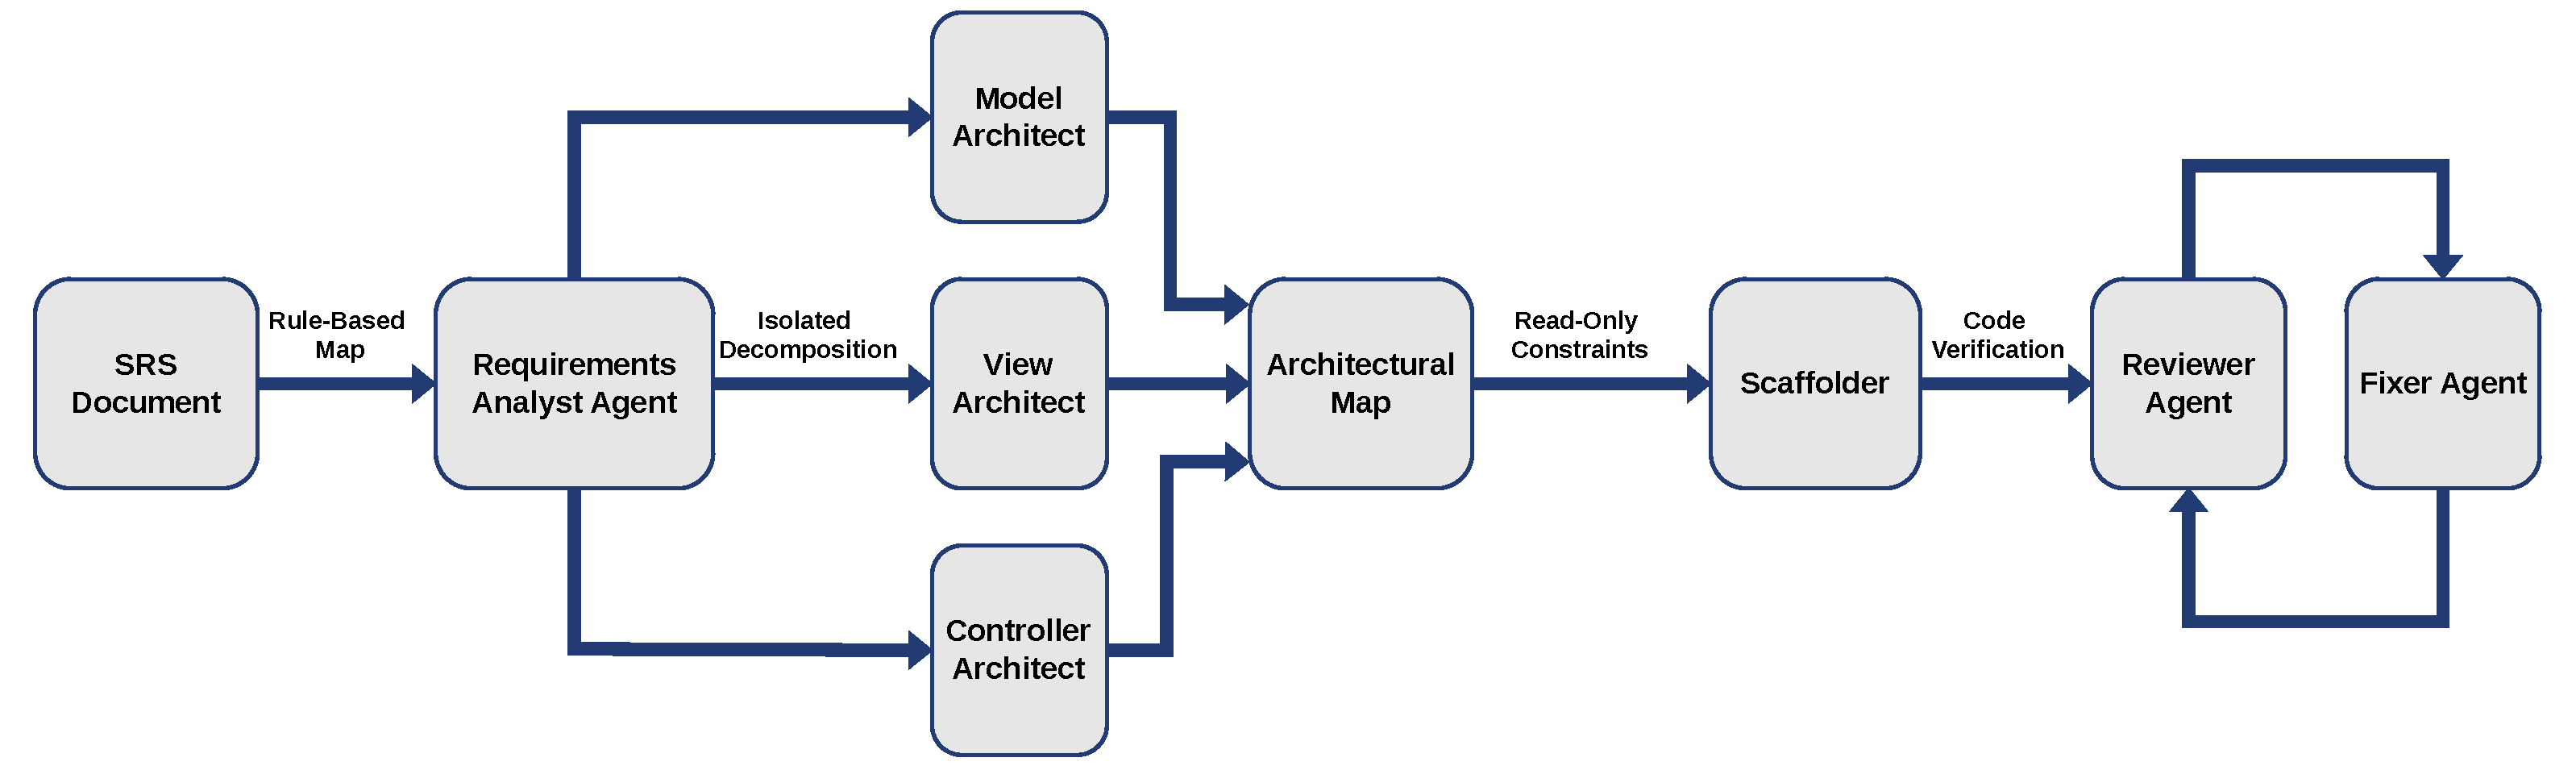
\includegraphics[width=0.80\linewidth]{images/Figure_1.pdf}
\caption{Architecture-First Multi-Agent Orchestration Pipeline. The SRS document is parsed by the Requirements Analyst Agent into a rule-based map, decomposed in isolation by three parallel Architect Agents (Model, View, Controller) into the Architectural Map, and passed as read-only constraints through the rule-based Scaffolder to a verification loop between the Reviewer Agent and Fixer Agent.}
\label{fig:31}
\end{figure}

Operationally, the system is governed by the fundamental ``Separation of Concerns'' principle, implemented through a sophisticated multi-agent topology. Rather than delegating complex, multi-faceted tasks to a single large model, the processes of planning, data extraction, code generation, and verification are decoupled into discrete domains with rigid boundaries. These responsibilities are distributed among highly specialized, independent AI agents. Throughout this paper, the term \textit{agent} refers exclusively to components that invoke an LLM to perform a bounded, task-specific function; the orchestrator, rule-based scaffolder, AST-based static analyzer, and human approval gate operate as rule-based control or analysis components. For instance, while the Requirements Analyst Agent is tasked exclusively with defining the domain taxonomy, the Architect Agents analyze and decompose the Model-View-Controller (MVC) layers in careful isolation. By using this systematic and modular taxonomy, each agent generates outputs constrained solely by its designated area of expertise. This isolation is designed to reduce the margin for hallucination and support the consistency of the generated artifacts under the tested configuration.

Data interoperability within this modular architecture is managed via the JSON format, providing a structured and machine-readable communication channel. This structured payload is designed to ensure that the architectural decisions synthesized by upstream agents serve as constraints for downstream phases. For example, the Architectural Map, generated independently by the Model Architect Agent, View Architect Agent, and Controller Architect Agent, defines the architectural perimeters that the Scaffolder is designed not to breach during code generation. In the final phase, the Reviewer Agent and Fixer Agent operate in tandem to verify that the generated implementation aims to adhere JSON-defined boundaries, autonomously remediating any detected deviations without compromising the initial architectural integrity. This cyclical, multi-agent interaction is designed to combine the stochastic generative capabilities of LLMs with the systematic, rule-based constraints of software engineering, thus establishing a sustainable and architecturally grounded development environment.

The effectiveness of this structured JSON communication protocol, a commonly used grounding strategy for reducing hallucination in LLM outputs, and the enforcement of architectural boundaries depends upon the precise semantic analysis of the initial requirements and their anchoring to a structured knowledge base. The mechanisms by which this critical prerequisite is fulfilled, and the process through which raw natural language data is transformed into structured architectural blueprints, are detailed in the subsequent phase.

\FloatBarrier
\subsection{Phase I: Automating Requirement Extraction: SRS Grounding and Domain Discovery}

The operational workflow for requirement extraction is depicted in Figure~\ref{fig:32}. In classical MVC-based development, the requirements analysis phase is where a human architect reads the specification documents, identifies the domain entities, and maps functional requirements to the Model, View, and Controller layers \citep{Reenskaug1979, Gamma1994}. Phase I automates this exact process. To ground every architectural decision in verified requirements and reduce the risk of hallucination, this phase employs Retrieval-Augmented Generation (RAG) \citep{Lewis2020}: rather than relying on the LLM's parametric knowledge, the system dynamically retrieves only the most semantically relevant SRS segments for each architectural query. Initiated via the \texttt{/extract} command, the operational lifecycle of the system begins with the ``SRS Grounding'' phase, which transforms raw textual inputs into structured, machine-actionable architectural data from which the overall structure of the project is derived.

\begin{figure}[pos=h]
\centering
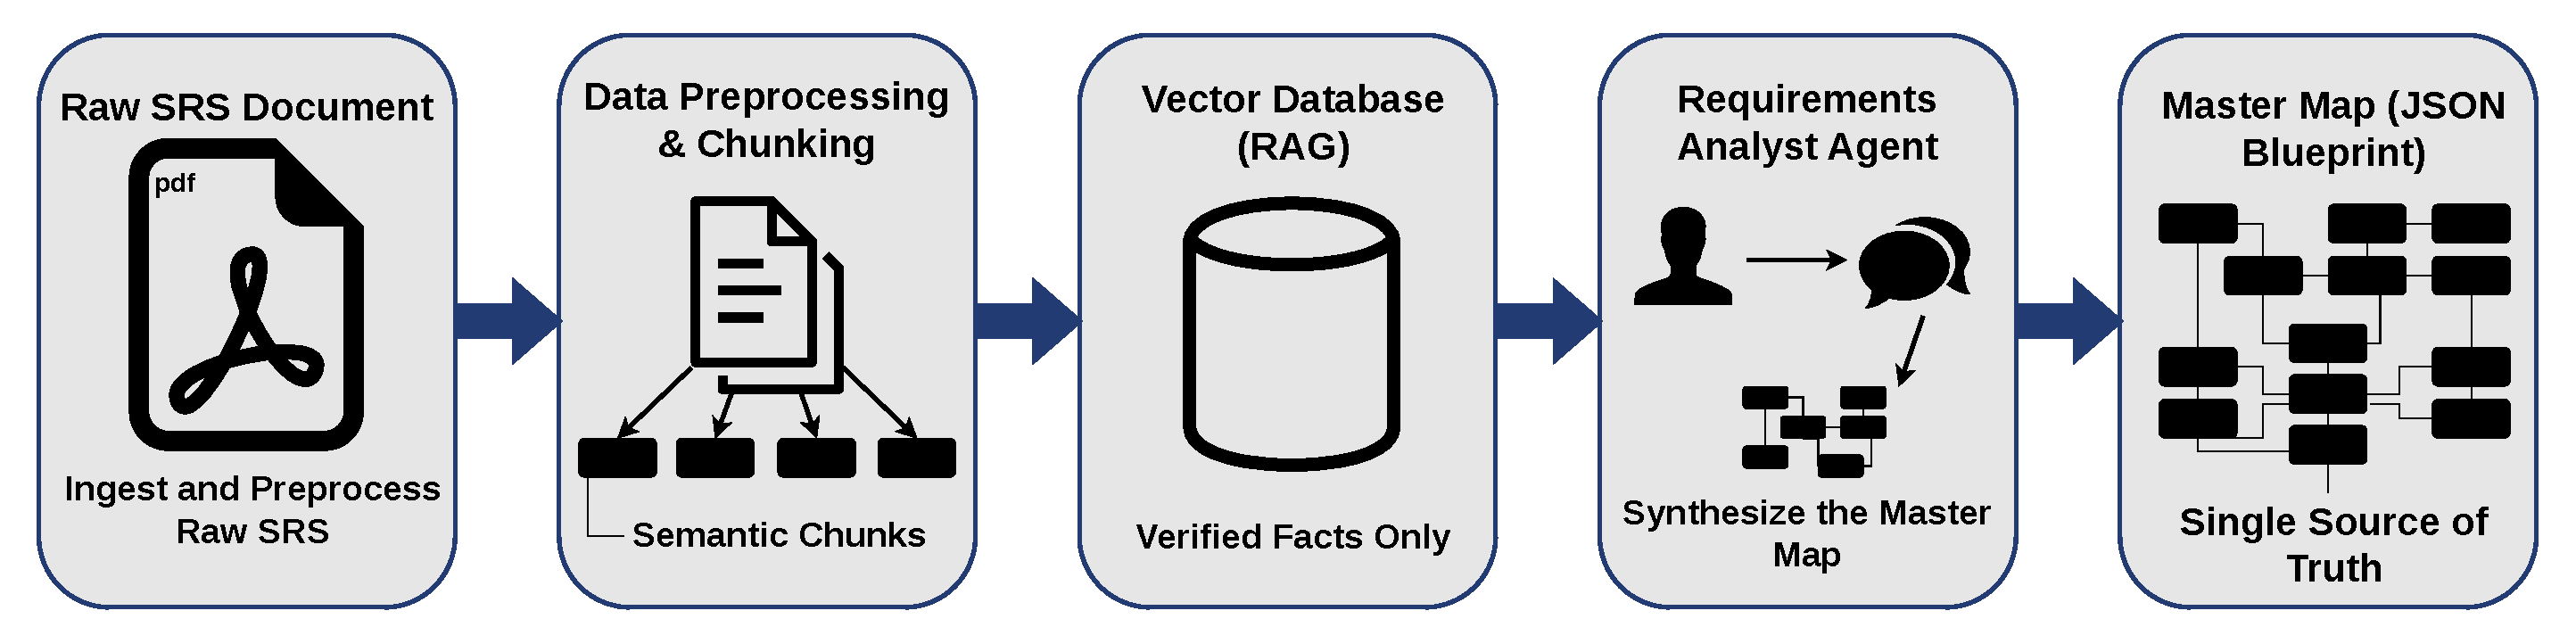
\includegraphics[width=0.80\linewidth]{images/Figure_2.pdf}
\caption{Phase I: SRS Grounding and Domain Discovery workflow. Raw SRS documents are preprocessed into semantic chunks, indexed in a Retrieval-Augmented Generation (RAG) vector database restricted to verified facts, and synthesized by the Requirements Analyst Agent into the Master Map, the system's single source of truth.}
\label{fig:32}
\end{figure}

During initialization, raw SRS documents (typically in PDF format) are ingested into the system. The extracted data undergoes systematic preprocessing to eliminate noise, encompassing format correction, whitespace trimming, and text normalization. The refined text is subsequently partitioned into overlapping segments (chunks) while aiming to preserve semantic integrity. This chunking strategy enables the system to focus exclusively on contextually relevant information blocks during downstream tasks, rather than repeatedly processing the entire document, which is intended to support extraction accuracy while reducing computational overhead.

The sanitized text segments are then embedded and indexed within a vector database, forming the operational core of the Retrieval-Augmented Generation (RAG) strategy. For any given architectural query, the system retrieves only the semantically most relevant SRS segments. By using this vector-based retrieval mechanism, the generative agents are guided to base their architectural synthesis primarily on verified facts. This strategic constraint aims to reduce the injection of fabricated features or hallucinated requirements, ensuring that the generated architectural scaffold remains as faithful as possible to the original specifications.

In the final step of the extraction pipeline, the system derives the Master Map. This artifact represents the formal transformation of complex natural language requirements into a structured ``project constitution'' comprehensible to the AI agents. During this synthesis, the Requirements Analyst Agent evaluates the extracted semantic data to define the foundational framework of the project.

Beyond serving as a high-level conceptual summary, the Master Map functions as a machine-readable, JSON-formatted blueprint detailing the project naming conventions, core data structures (Domain Entities), and primary operational capabilities (System Functions). This blueprint acts as the system's single source of truth. Consequently, all downstream Architect Agents tasked with synthesizing the Model, View, and Controller layers generate their respective class definitions by referencing this centralized map.

This methodology provides a key advantage: it aims to prevent the AI from arbitrarily introducing unnecessary features or unverified logic into the project. Because the functional scope and data constraints are explicitly defined at the project's inception, the system strives to maintain a consistent traceability chain between the initial natural language requirements, the intermediate class structures, and the final source code. This end-to-end traceability promotes consistent and reproducible behavior across all system components throughout the development lifecycle.

Although the Master Map establishes the conceptual foundation of the project, this centralized blueprint is subsequently decomposed in accordance with MVC principles to synthesize a functional software architecture. The subsequent section details how the Model, View, and Controller layers are autonomously constructed in an isolated manner, using this centralized blueprint as their foundational premise.

Large Language Models (LLMs) are used in the extraction phase to overcome semantic ambiguity in SRS documents. Unlike traditional rule-based Natural Language Processing (NLP), which relies on strict syntactic parsing, the LLM acts as a semantic synthesizer. It grasps the broader context to map scattered functional requirements directly into a structured MVC architecture.

In summary, Phase I takes a raw SRS document as input and produces two key outputs: a RAG-indexed vector database of semantically chunked requirements, and the \texttt{requirements\_analysis.json} artifact (Table~\ref{tab:artifact_flow})---a structured JSON blueprint defining the project's domain entities and system functions. This artifact serves as the single source of truth for all downstream agents and is consumed directly by the three Architect Agents in Phase II to decompose the architecture into isolated Model, View, and Controller components.

\FloatBarrier
\subsection{Phase II: Automating Architectural Design: Agent-Driven MVC Component Extraction}
\label{sec:phase2}

The systematic decomposition of the architectural layers is illustrated in Figure~\ref{fig:33}. This phase implements the architectural design process, facilitating the systematic transformation of the Master Map into a concrete Model-View-Controller (MVC) software architecture. The primary objective is to separate abstract architectural reasoning from concrete code generation as cleanly as possible. Consequently, the specifications for each MVC layer are formalized into structured JSON artifacts, bounded by their respective architectural responsibilities. This decomposition is orchestrated by three highly specialized generative agents, the Model, View, and Controller Architect Agents, which aim to enforce the isolation of the system's data structures, presentation layers, and business logic, respectively.

\begin{figure}[pos=h]
\centering
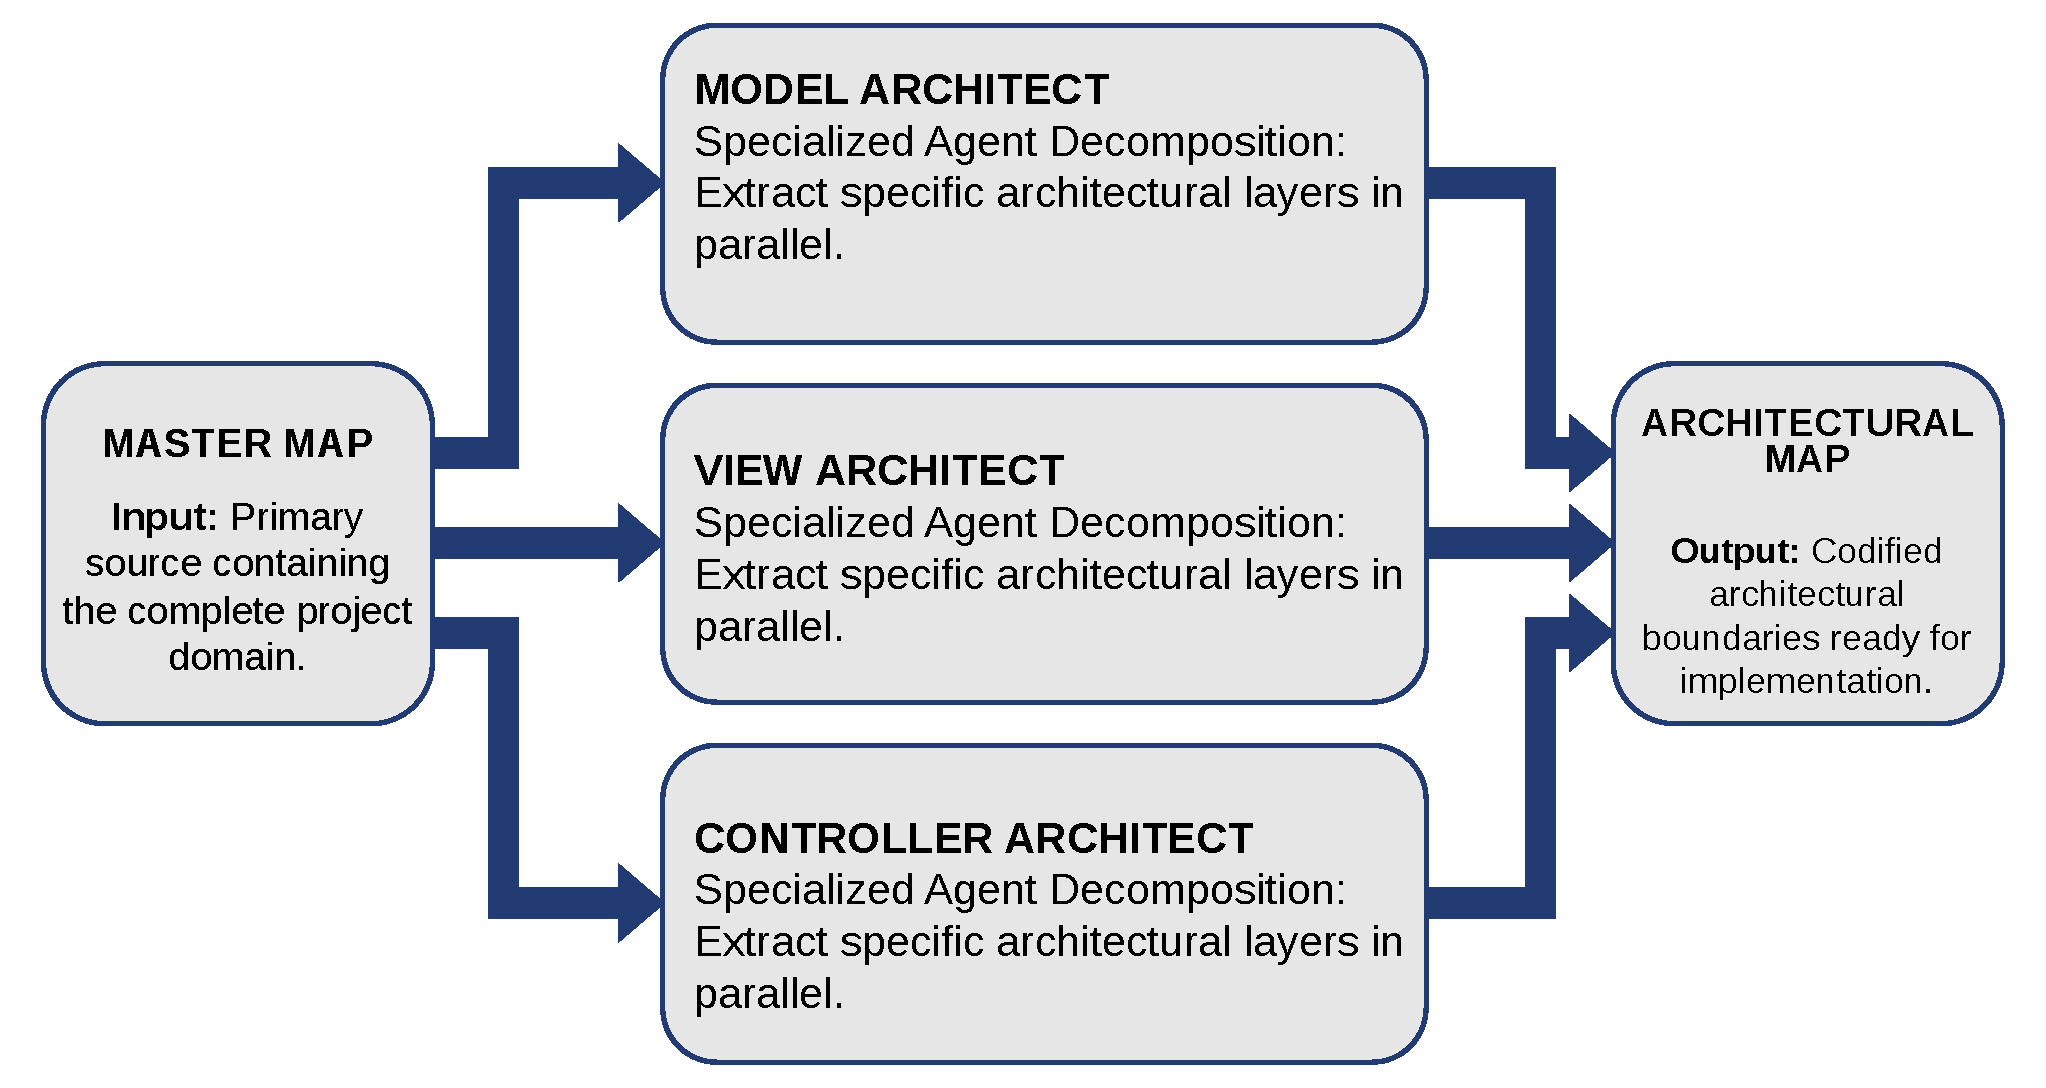
\includegraphics[width=0.80\linewidth]{images/Figure_3.pdf}
\caption{Phase II: Agent-Driven MVC Component Extraction process. The Master Map is decomposed in parallel by three specialized Architect Agents, Model, View, and Controller, each extracting its respective architectural layer, and the resulting outputs are consolidated into the Architectural Map, a structured Model-View-Controller (MVC) JSON artifact ready for implementation.}
\label{fig:33}
\end{figure}

In classical MVC development, formalizing the Model layer is the data architect's responsibility: they manually define domain entities' attributes, data types, and inter-entity relationships, typically through entity-relationship or Unified Modeling Language (UML) class diagrams \citep{Gamma1994}. The Domain Entity Modeling phase automates this exact process. During this phase, the Model Architect Agent autonomously identifies and extracts the core domain entities from the Master Map. To prevent unnecessary complexity and keep the architectural scope manageable, this extraction is capped at a maximum of eight core entities, an implementation limit chosen to bound prompt and artifact size during this feasibility evaluation. These caps are prototype constraints rather than theoretically optimal MVC sizes. Consequently, the system aims to focus the data backbone on the most critical business objects. The resulting JSON artifact explicitly defines the names and functional attributes of each entity, formally establishing the project's semantic data model.

In classical MVC development, the Controller layer is the human architect's responsibility: they manually define which business workflows map to which controller actions, ensuring that the Model and View remain decoupled \citep{Gamma1994}. The Behavioral Logic Mapping phase automates this exact responsibility. Here, the Controller Architect Agent analyzes the documented workflows to synthesize a maximum of six controllers, each constrained to 3–5 specific actions. The most critical constraint enforced during this phase is the ``Zero-Inference'' policy. This heuristic prohibits the agent from autonomously injecting default Create, Read, Update, Delete (CRUD) operations unless they are explicitly mandated by the underlying SRS document. By preventing the generative tendency to hallucinate unnecessary features, this policy aims to preserve architectural fidelity.

Finally, in classical MVC development, the View layer is the interface designer's responsibility: they manually derive the required screens and navigation paths from the documented user journeys \citep{Gamma1994}. The Presentation Layer Abstraction phase automates this exact responsibility, defining the system's interface boundaries. The View Architect Agent synthesizes up to six primary user interfaces based on the extracted user journeys, an implementation limit consistent with the prototype's output-budget constraints, defining solely their functional names and intended purposes. This phase is likewise governed by the ``Zero-Inference'' policy introduced above: the View Architect Agent is prohibited from fabricating screens or interface elements that are not grounded in the extracted user journeys. Crucially, low-level user interface components (e.g., specific buttons, sliders, or graphical widgets) are intentionally abstracted away. This high-level approach allows that the system defines its functional navigation and presentation logic without incurring the overhead of implementation-specific visual details.

In summary, Phase II takes the \texttt{requirements\_analysis.json} artifact produced in Phase I as input and produces the \texttt{architecture\_map.json} artifact (Table~\ref{tab:artifact_flow}), which formally codifies the system's domain entities, controller actions, and user interface boundaries across the three MVC layers. This artifact serves as the architectural constraint for the Scaffolder in Phase III, which translates this abstract design into a concrete, rule-based file system structure.

\FloatBarrier
\subsection{Phase III: Automating Implementation: Rule-Based Scaffolding and Code Generation}
\label{sec:phase3}

In classical MVC development, the implementation phase is where a human developer manually creates the directory structure, writes the class skeletons for each layer, and populates them with business logic, typically guided by the architectural blueprint defined in the design phase \citep{Gamma1994}. Phase III automates this exact workflow through two sequential steps. The transition from architectural abstraction to physical implementation is shown in Figure~\ref{fig:34}. This phase encompasses the implementation stage, wherein the structured JSON artifacts derived in Section~\ref{sec:phase2} are translated into concrete source code. Rather than relying on stochastic, end-to-end code generation, this conversion follows a structured two-step protocol designed to preserve structural integrity. By systematically translating architectural decisions into codebase-level structures, this process aims to reduce the risk of architectural drift between the abstract design and the physical implementation.


The Rule-Based Project Scaffolding step acts as a critical safety perimeter, bridging the abstract architectural blueprint and the concrete file system. Initiated via the \texttt{/scaffold} command, the project's directory hierarchy and foundational class skeletons are synthesized using strict, rule-based algorithms, entirely independent of LLM intervention. This rule-based execution is designed to ensure that all file names, class definitions, and directory trees align with the predefined architectural artifacts. Consequently, structural inconsistencies at the file system level are reduced, providing the developer with a structurally aligned project scaffold intended to support MVC compliance with the SRS.

\begin{figure}[pos=h]
\centering
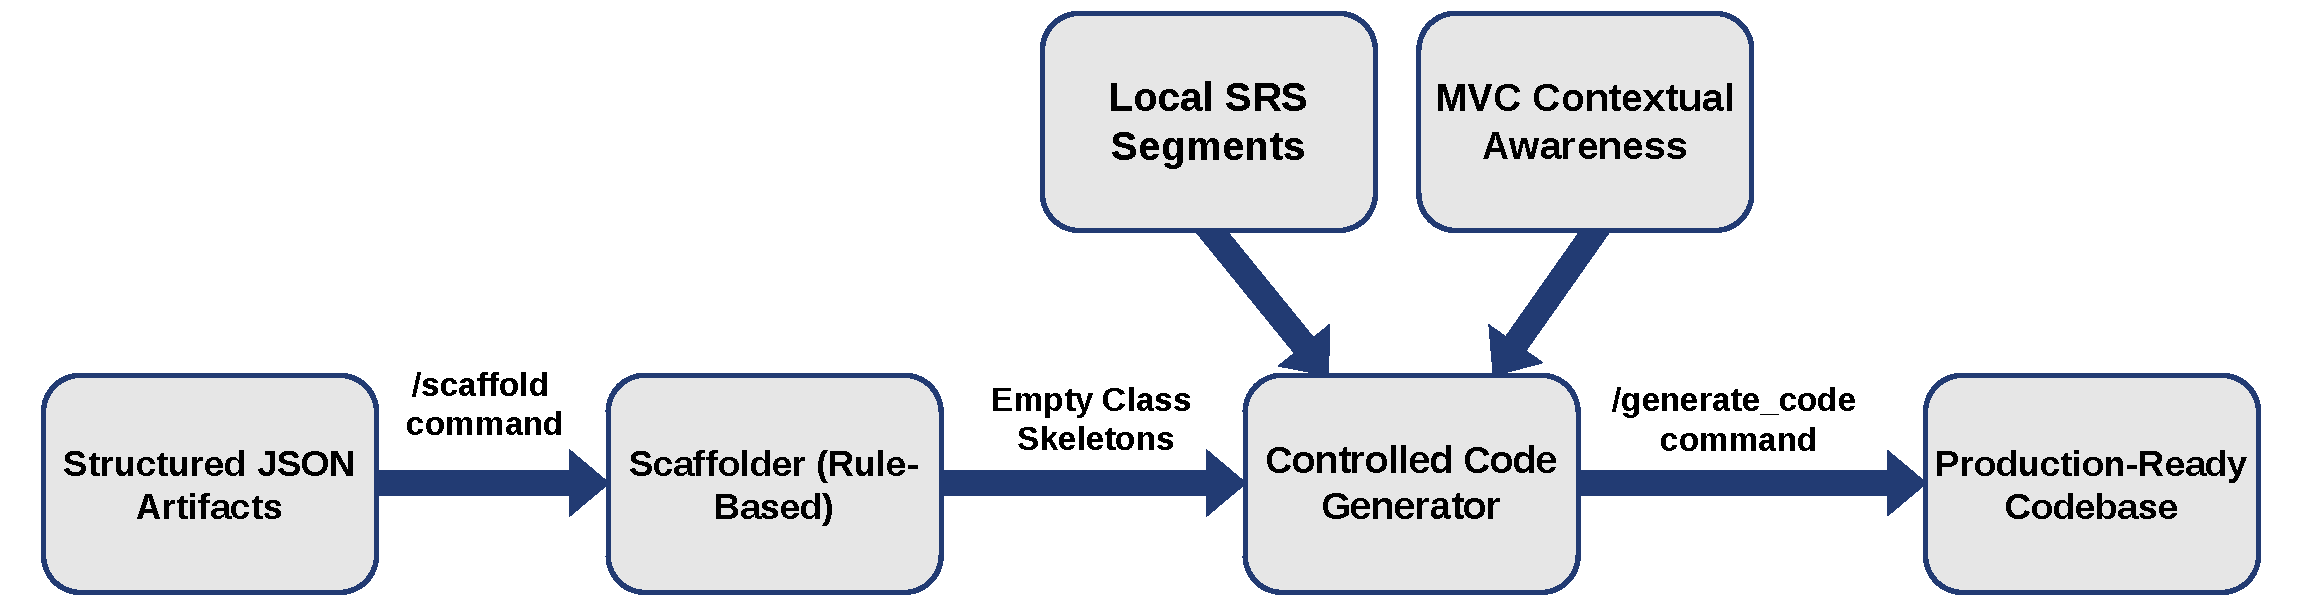
\includegraphics[width=0.80\linewidth]{images/Figure_4.pdf}
\caption{Phase III: Rule-Based Scaffolding and Code Generation workflow. The Structured JSON Artifacts are converted into empty class skeletons by the rule-based Scaffolder via the \texttt{/scaffold} command, which are then populated with Local SRS Segments and MVC Contextual Awareness by the Controlled Code Generator via the \texttt{/generate\_code} command to produce the production-ready codebase.}
\label{fig:34}
\end{figure}

The Code Generation step then populates these empty scaffolds with the actual implementation. Initiated via the \texttt{/generate\_code} command, the developer orchestrates the implementation of specific layers (Model, View, or Controller) by synthesizing contextual data from both the global architectural blueprint and the localized SRS segments. This methodology transitions code generation from a stochastic output model into a highly controlled workflow, tightly constrained by a pre-validated architectural framework.

A critical architectural checkpoint emerges during the generation of the Controller logic. For a controller to orchestrate data flow accurately, it requires contextual awareness of the data it manipulates (Model) and the interfaces it serves (View). To enforce this MVC principle, the code generation pipeline provides the generative agent with explicit, read-only access to these inter-layer relationships, ensuring functional cohesion.

In scenarios where the underlying SRS document exhibits ambiguities or underspecified details, the system is constrained to derive logical inferences solely from the established architectural taxonomy, rather than hallucinating spurious functionalities. By drawing on industry-standard ``reasonable defaults,'' the system synthesizes the missing business logic in a manner that remains consistent with the project's overarching architectural intent.

In summary, Phase III takes the \texttt{architecture\_map.json} artifact from Phase II (Table~\ref{tab:artifact_flow}) as input and produces two outputs: a rule-based project scaffold defining the directory structure and class skeletons, and an LLM-generated implementation constrained by the Architectural Map and SRS segments. The resulting codebase targets Python engineering standards (e.g., PEP 8) and static typing, aiming to provide a structured and maintainable foundation. However, since LLM-based generation is inherently stochastic, the generated code is passed directly to Phase IV, where it is audited for MVC compliance and any detected violations are autonomously remediated.

\subsection{Phase IV: Automating Code Review: MVC-Based Auditing and Autonomous Remediation Loop}

In classical MVC development, ensuring that an implementation respects layer boundaries is the human reviewer's responsibility: code review is where violations such as a View directly accessing a Model are caught before integration \citep{Gamma1994}. Phase IV automates this exact responsibility, extended in this study to include violation categories specific to this system's Controller-centric design, such as business logic displaced outside the Controller (Section~\ref{sec:experiment}). The autonomous verification and remediation cycle is illustrated in Figure~\ref{fig:35}. This phase, characterized by autonomous error detection and self-healing capabilities, represents one of the principal contributions of the \textit{MVC Test Orchestrator}. Beyond generating architecturally compliant scaffolds and implementations, the system continuously monitors the codebase for adherence to the predefined architectural constraints. By filtering stochastic LLM outputs through a rule-based validation mechanism, this phase detects and repairs selected MVC layer violations in the generated artifacts.

\begin{figure}[pos=h]
\centering
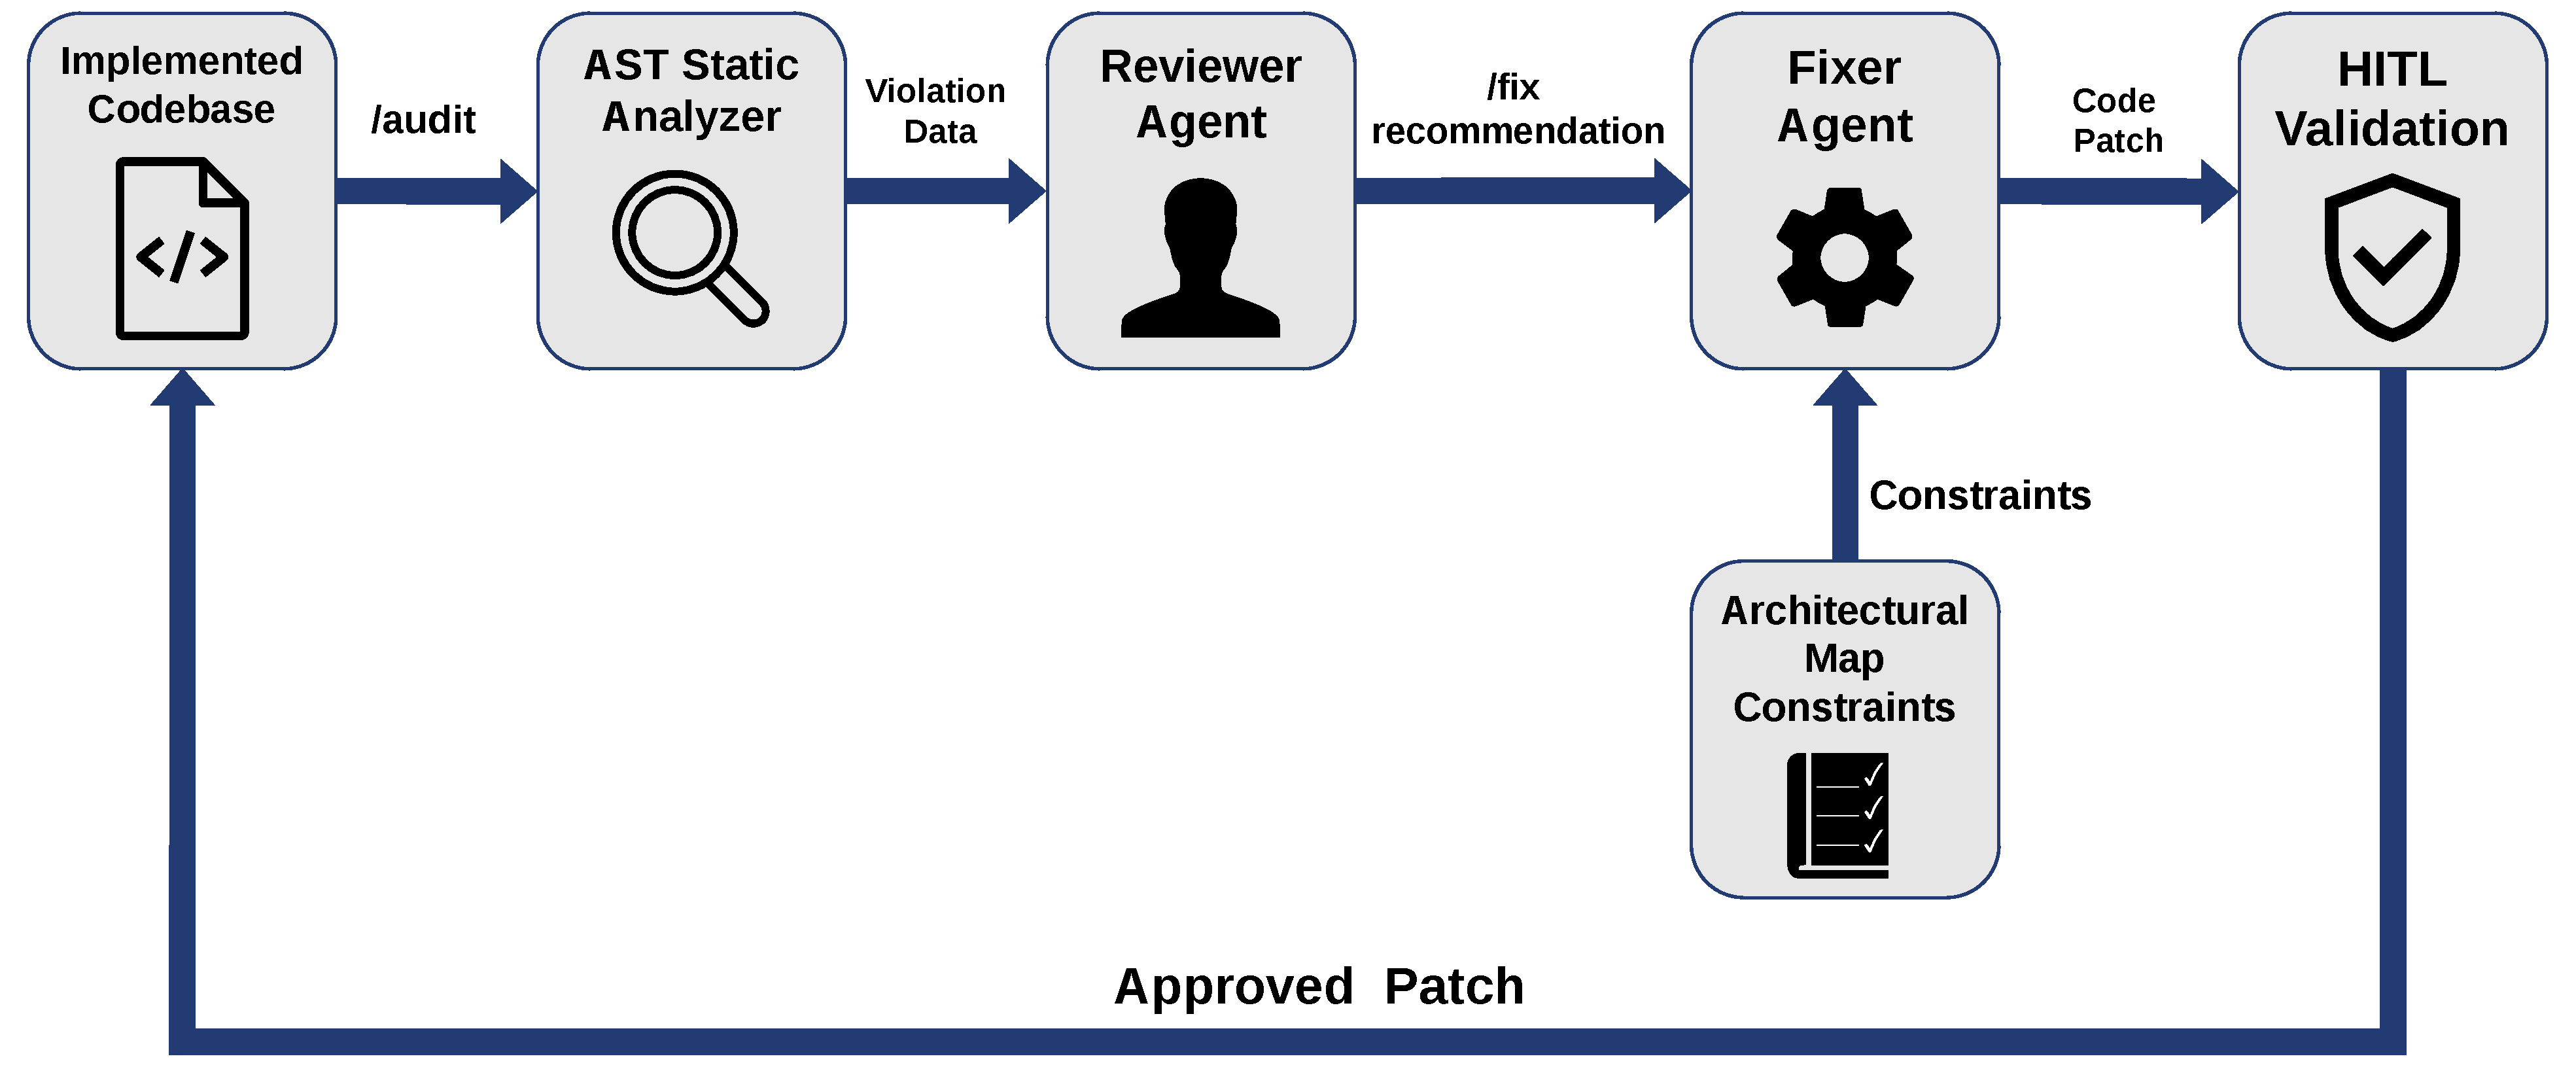
\includegraphics[width=0.80\linewidth]{images/Figure_5.pdf}
\caption{Phase IV: Automated Auditing and Self-Healing Loop. The implemented codebase is inspected by the Abstract Syntax Tree (AST) Static Analyzer via the \texttt{/audit} command, whose violation data is triaged by the Reviewer Agent; the Fixer Agent then patches the code under Architectural Map constraints via the \texttt{/fix} recommendation, subject to Human-in-the-Loop (HITL) validation before the approved patch returns to the codebase.}
\label{fig:35}
\end{figure}

The core of this validation mechanism is a rule-based static analysis framework built upon Abstract Syntax Tree (AST) parsing. Triggered via the \texttt{/audit} command, this module comprehensively inspects the implemented codebase, verifying both syntactic validity and adherence to inter-layer dependency constraints. For instance, MVC isolation violations, such as a View component directly instantiating or querying a Model object, are statically detected prior to execution. The analyzer implements four bounded, syntax-directed checks over Python ASTs combined with pattern-based rules; it is not a general semantic defect detector.

Detected violations are aggregated into a structured, machine-readable feedback report, which the Reviewer Agent uses to synthesize concrete, actionable refactoring strategies to resolve the identified violations.

The culmination of the validation process is the constrained remediation phase, initiated via the \texttt{/fix} command. Operating on the telemetry provided by the \texttt{/audit} report, the Fixer Agent autonomously patches the defective code blocks while aiming to preserve architectural integrity. This remediation is explicitly ``constrained'' because the generative agent treats the Architectural Map and the rule-based project scaffold as read-only, restricting its edits to the flagged code blocks alone. This limitation minimizes the risk of introducing secondary structural regressions while resolving an isolated bug. Ultimately, the \texttt{/fix} mechanism integrates automated repair with a Human-in-the-Loop (HITL) protocol, requiring developer validation before committing the proposed architectural patches.

In summary, Phase IV takes the generated codebase from Phase III as input and produces two outputs: the \texttt{violations.json} artifact (Table~\ref{tab:artifact_flow}) detailing all detected MVC layer breaches, and a patched codebase in which identified violations have been autonomously remediated by the Fixer Agent within the boundaries of the \texttt{architecture\_map.json} artifact. The patched code is then presented to the developer for final validation through the HITL protocol, which governs the strategic oversight of all four phases and is described in the following subsection.


\subsection{Human-in-the-Loop (HITL) Integration}

The balanced interaction between human expertise and automated processes is depicted in Figure~\ref{fig:36}. The proposed methodology embeds human strategic governance into the generative loop. Rather than functioning as an opaque, fully autonomous black-box, the \textit{MVC Test Orchestrator} implements a structured Human-in-the-Loop (HITL) paradigm. This architecture formalizes an iterative control mechanism between the developer and the multi-agent system. At its core, this approach provides checkpoints at which a developer may inspect, reject, or edit intermediate artifacts before the pipeline advances, offering a mechanism to align the generative throughput of LLMs with the strategic oversight and judgment of human software engineers.

\begin{figure}[pos=h]
\centering
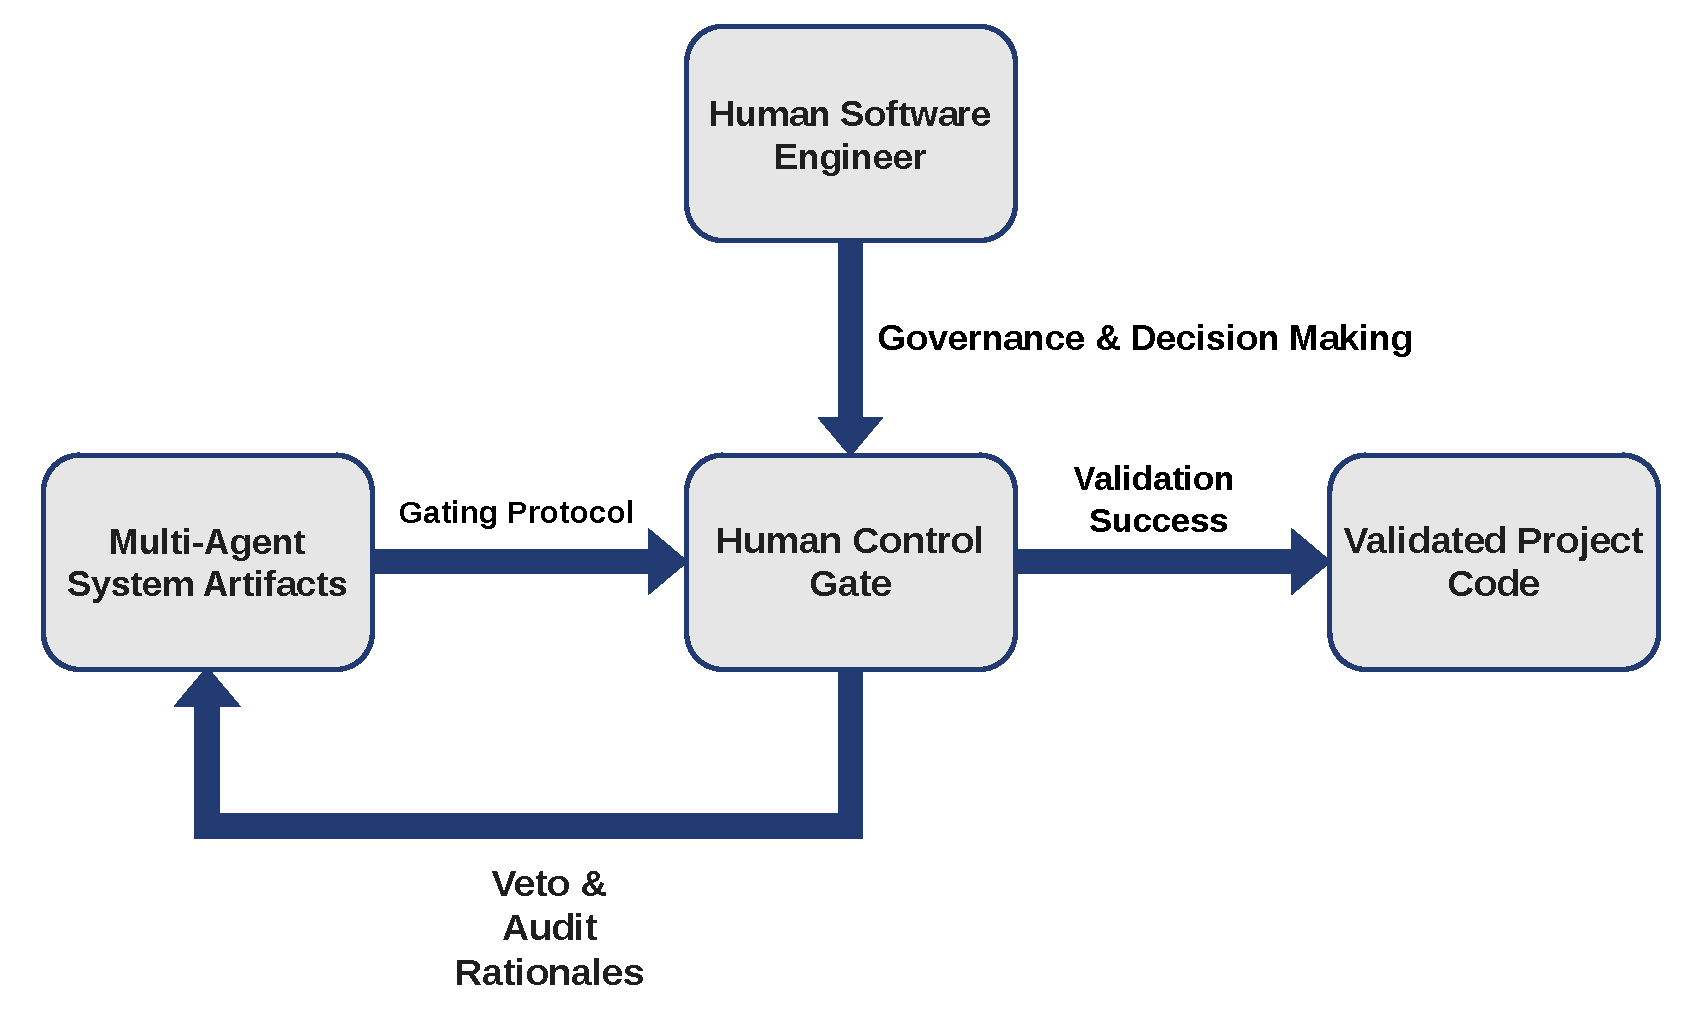
\includegraphics[width=0.62\linewidth]{images/Figure_6.pdf}
\caption{Strategic Human-in-the-Loop Governance Protocol. The Human Software Engineer exercises governance over the Human Control Gate, which admits Multi-Agent System Artifacts through a gating protocol and either validates them into approved project code or returns veto and audit rationales back to the artifacts for revision.}
\label{fig:36}
\end{figure}

The HITL mechanism acts as a structured gating protocol at critical points within the pipeline. The developer retains the authority to inspect, modify, or veto the system's outputs at every phase, from the initial JSON-based architectural scaffolding to the final AST-driven code review. Furthermore, the explainable, natural-language rationales generated during the \texttt{/audit} and \texttt{/fix} phases equip developers with the necessary context to objectively evaluate the AI's technical recommendations. By bounding AI autonomy within this collaborative framework, the system helps reduce cascading structural errors within the generated codebase. Ultimately, preserving developer sovereignty over the project supports a development lifecycle that is both architecturally resilient and industrially viable.

\subsection{Inter-Phase Artifact Summary}

Each pipeline phase produces a structured, machine-readable artifact that serves as the sole communication contract between successive agents. Table~\ref{tab:artifact_flow} consolidates these artifacts: the phase in which each is generated (with a reference to the corresponding workflow figure), its contents, and the downstream component that consumes it. This table is used as the unified reference throughout Section~\ref{sec:experiment} and Section~\ref{sec:results}, replacing repeated inline file-name citations.

% --- ARTIFACT FLOW TABLE ---
\begin{table}[pos=h]
\centering
\caption{Inter-phase artifact flow: structured outputs generated and consumed across pipeline phases.}
\label{tab:artifact_flow}
\renewcommand{\arraystretch}{1.3}
\begin{tabularx}{\textwidth}{@{} >{\raggedright\arraybackslash}X l >{\raggedright\arraybackslash}X >{\raggedright\arraybackslash}X @{}}
\toprule
\textbf{Artifact (File Name)} & \textbf{Generated In} & \textbf{Contents} & \textbf{Used In} \\
\midrule
Requirements Analysis Artifact \newline (\texttt{requirements\_analysis.json}) & Phase I (Fig.~\ref{fig:32}) & Extracted domain entities and system functions synthesized from the SRS by the Requirements Analyst Agent & Phase II --- Architect Agents \\
\midrule
Architectural Map Artifact \newline (\texttt{architecture\_map.json}) & Phase II (Fig.~\ref{fig:33}) & MVC component definitions (Model, View, Controller) produced by the three Architect Agents & Phase III --- Scaffolder \\
\midrule
Scaffolded Codebase Artifact & Phase III (Fig.~\ref{fig:34}) & MVC directory structure with class skeletons and template files generated systematically from \texttt{architecture\_map.json} & Phase IV --- AST-based static analyzer \\
\midrule
Violation Report Artifact \newline (\texttt{violations.json}) & Phase IV (Fig.~\ref{fig:35}) & Detected architectural violations with severity levels produced by the AST-based static analyzer & Phase IV --- Fixer Agent \\
\bottomrule
\end{tabularx}
\end{table}